\documentclass[12pt, titlepage]{report}
\usepackage{consumer_resource_final}
\graphicspath{{./figures/}}

\begin{document}
% \subsection{Time evolution}
% \begin{figure}[h!]
% \centering
% 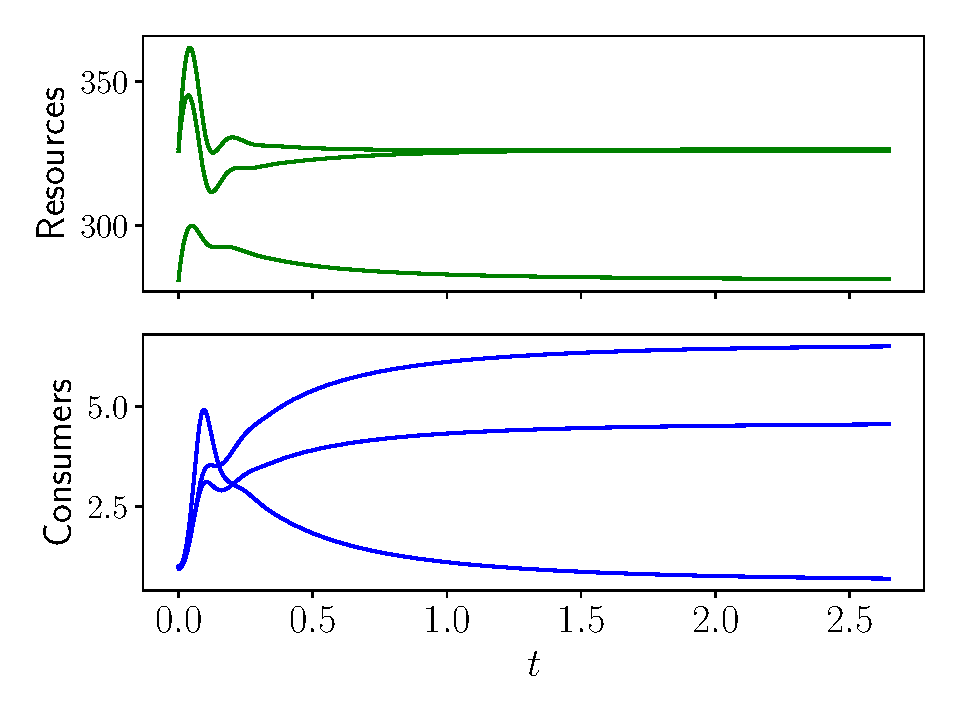
\includegraphics[width=0.6\linewidth]{Typical_time_evolution/Typical_time_evolution_resources_species_high_threshold.pdf}
% \caption{Time evolution for high coefficient threshold ($\epsilon_{\text{conv}}=10^{-1}$)}
% 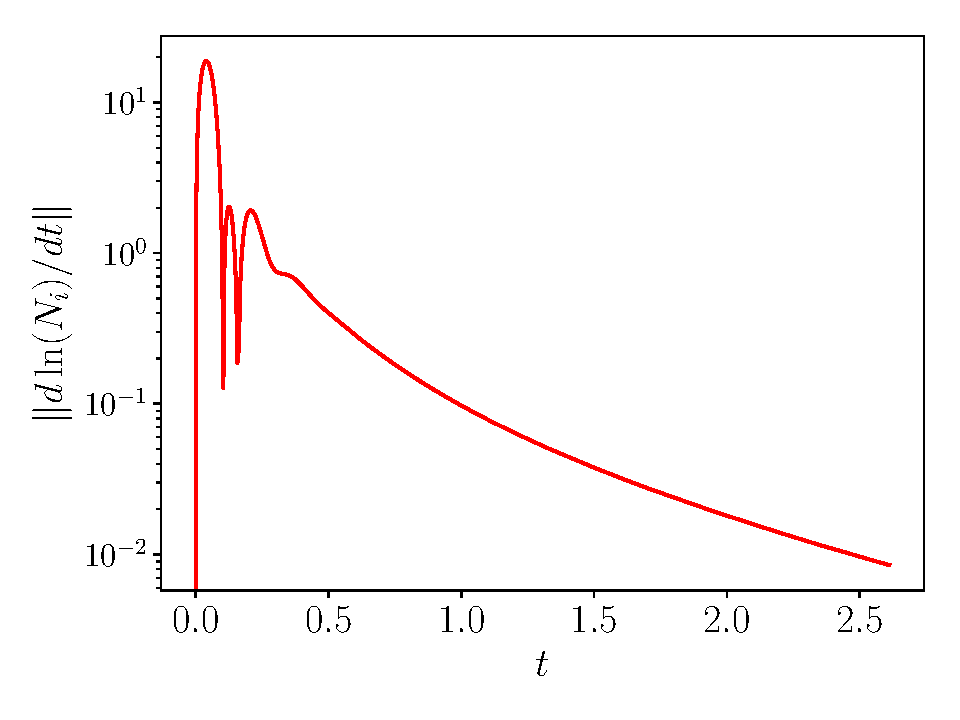
\includegraphics[width=0.6\linewidth]{figures/Typical_time_evolution/Typical_time_evolution_log_derivative_high_threshold.pdf}
% \caption{Typical convergence to judge equilibrium, we see the simulation stops at $\epsilon_{\text{conv}}=10^{-1}$}
% \end{figure}
% \begin{figure}[h!]
% \centering
% 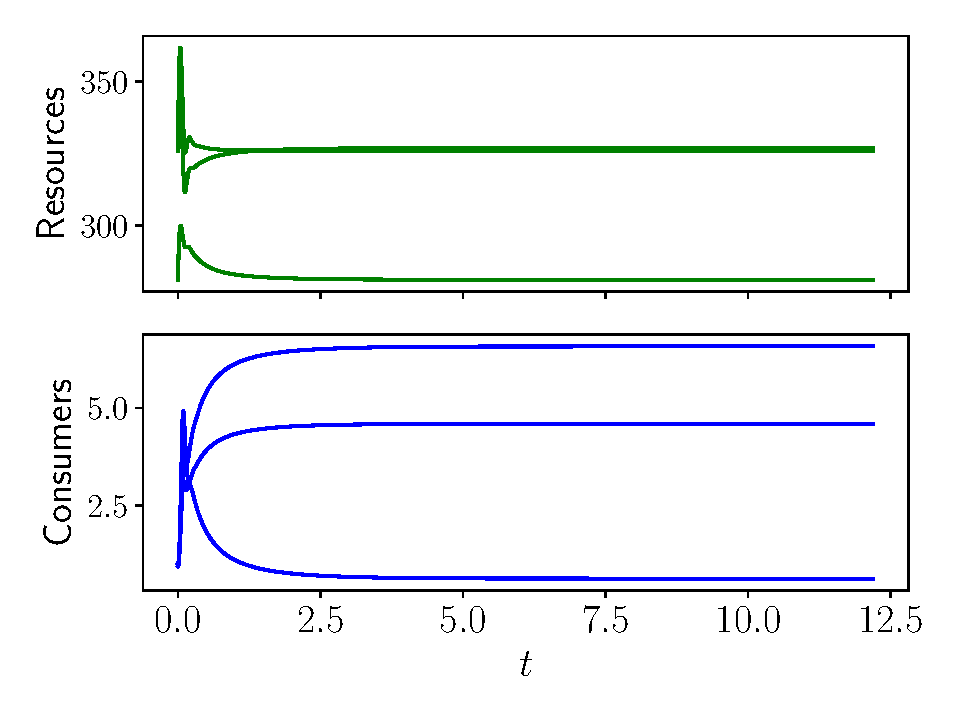
\includegraphics[width=0.6\linewidth]{Typical_time_evolution/Typical_time_evolution_resources_species_low_threshold.pdf}
% \caption{Time evolution for low coefficient threshold (more accuracy) ($\epsilon_{\text{conv}}=10^{-5}$)}
% 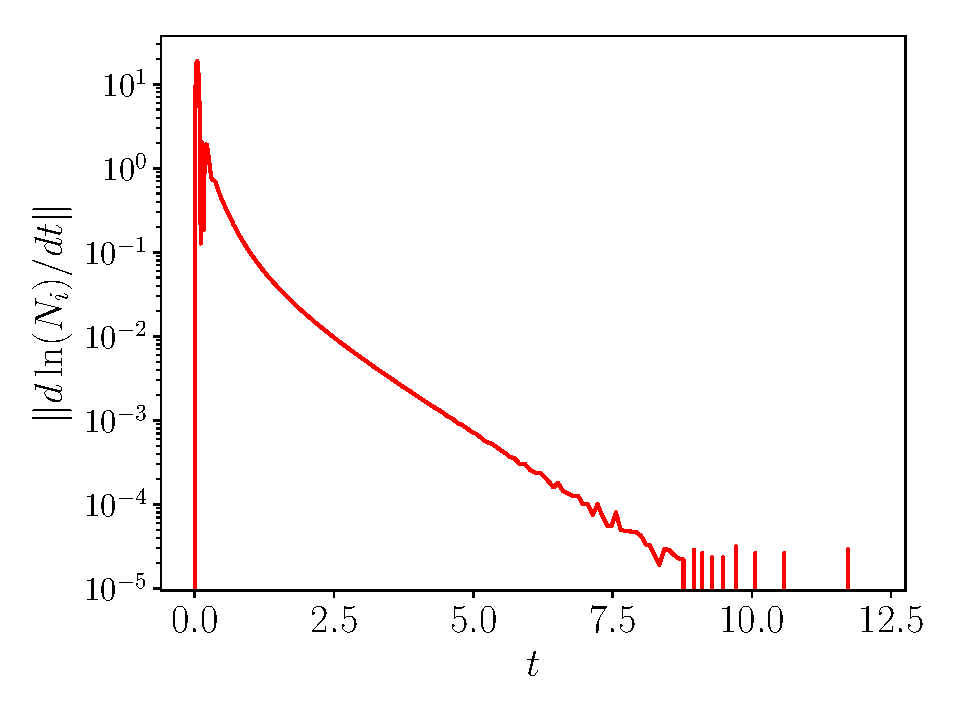
\includegraphics[width=0.6\linewidth]{figures/Typical_time_evolution/Typical_time_evolution_log_derivative_low_threshold.pdf}
% \caption{Typical convergence to judge equilibrium, we see the simulation stops at $\epsilon_{\text{conv}}=10^{-5}$}
% \end{figure}
% \subsection{Allowed parameters : syntrophy range}
% \begin{figure}[h!]
% \centering
% 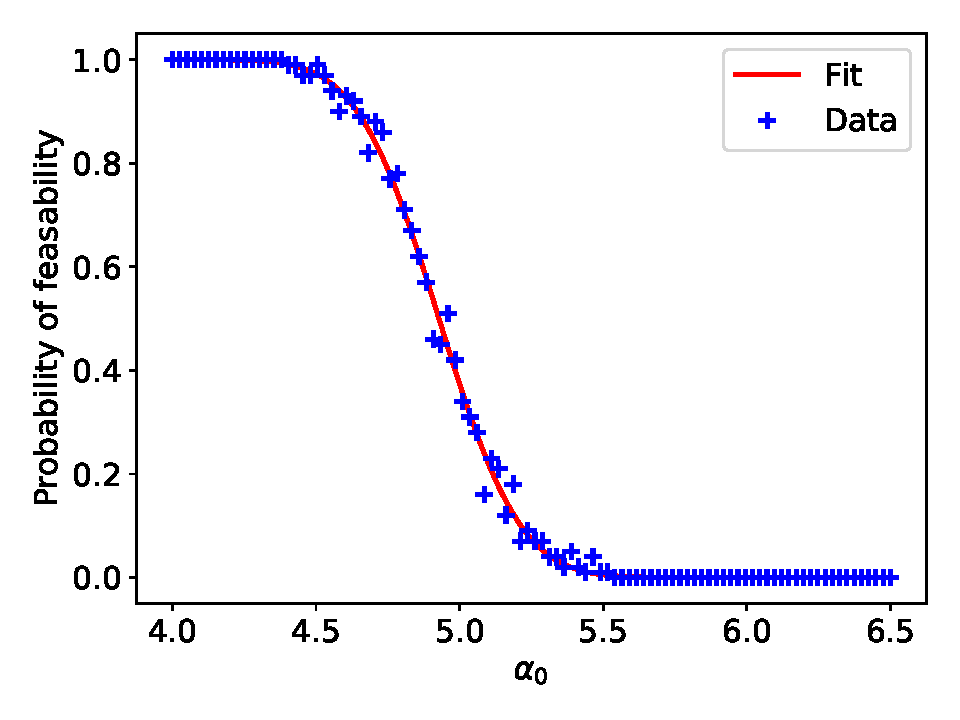
\includegraphics[scale=0.7]{figures/alpha0_probability_of_feasability}
% \caption{Typical shape of the probability of feasability for every metaparameter fixed except varying $\alpha_0$. We see that the probability of drawing a feasible system decreases sharply as $\alpha_0$ increases. A typical sigmoidal curve (here an erf function) fits the numerical data quite well.}
% \end{figure}

% \subsection{Studying the impact of the food network structure}
% \subsection{Studying the impact of syntrophy}
% We run a bunch of simulations with the following metaparameters. We made sure that these are compatible with the bounds on $\alpha_0$ Eqs.\eqref{eq : alpha bounds}.
%
% % Please add the following required packages to your document preamble:
% % \usepackage{graphicx}
% \begin{table}[h!]
% \centering
% \begin{tabular}{c|c|c|c|c|c}
% $\gamma_0$ & $\sigma_0$ & $\alpha_0$ & $R_0$ & $S_0$ & $l_0$ \\ \hline
% 1          & 1          & 0          & 300   & 1     & 11091 \\
%          & 0.75       & 0          &       &       &       \\
%          &            & 0.5        &       &       &       \\
%          & 0.5        & 0          &       &       &       \\
%          &            & 0.5        &       &       &       \\
%          &            & 1          &       &       &       \\
%          & 0.25       & 0          &       &       &       \\
%          &            & 0.5        &       &       &       \\
%          &            & 1          &       &       &       \\
%          &            & 1.5        &       &       &
% \end{tabular}
% \caption{Metaparameters used for the simulations.} \label{eq : table metaparameters used}
% \end{table}

\subsection{LRI regime}
\subsubsection{Outcome of the Monte Carlo algorithm}

\subsection{Fully dynamically stable volume}
\begin{figure}
\vspace{-120pt}
\hspace{-0.1\linewidth}
\subfloat[]{\includegraphics[width=1.2\linewidth]{{local_dynamical_stability_wt_wc_region_NR25_NS25_Nest0.35_Conn0.2208}.pdf}}

\vspace{-68pt}
\hspace{-0.1\linewidth}
\subfloat[]{\includegraphics[width=1.2\linewidth]{{local_dynamical_stability_wt_wc_region_NR25_NS25_Nest0.35_Conn0.3216}.pdf}}

\vspace{-68pt}
\hspace{-0.1\linewidth}
\subfloat[]{\includegraphics[width=1.2\linewidth]{{local_dynamical_stability_wt_region_NR25_NS25_Nest0.35_Conn0.272}.pdf}}

\caption{}
\end{figure}

\end{document}
